\documentclass[a4paper,12pt]{article}
\usepackage[english,ukrainian,russian]{babel}
\linespread{1}
\usepackage{ucs}
\usepackage[utf8]{inputenc}
\usepackage[T2A]{fontenc}
\usepackage[paper=portrait,pagesize]{typearea}
\usepackage{amsmath}
\usepackage{bigints}
\usepackage{amsfonts}
\usepackage{graphicx}
\usepackage{amssymb}
\usepackage{cancel}
\usepackage{gensymb}
\usepackage{multirow}
\usepackage{rotate} 
\usepackage{pdflscape}
\usepackage{bigstrut}
\usepackage[pageanchor]{hyperref}
\usepackage{chngpage}
\newcommand{\dx}{\textbf{d}x}
\newcommand{\dt}{\textbf{d}t}
\newcommand{\du}{\textbf{d}u}
\newcommand{\dv}{\textbf{d}v}
\newcommand{\dy}{\textbf{d}y}
\newcommand{\ds}{\textbf{d}s}
\newcommand{\dz}{\textbf{d}z}
\newcommand{\arch}{\textrm{arcch}}
\newcommand{\arsh}{\textrm{arcsh}}
\newcommand{\dint}{\displaystyle\int}
\newcommand\tab[1][1cm]{\hspace*{#1}}
\newcommand{\dsum}{\displaystyle\sum}
\usepackage[left=20mm, top=20mm, right=15mm, bottom=15mm, nohead, nofoot]{geometry}
\usepackage{verbatim}

\usepackage{listings}
\usepackage{xcolor}

\definecolor{codegreen}{rgb}{0,0.6,0}
\definecolor{codegray}{rgb}{0.5,0.5,0.5}
\definecolor{codepurple}{rgb}{0.58,0,0.82}
\definecolor{backcolour}{rgb}{0.95,0.95,0.92}

\lstdefinestyle{mystyle}{
	backgroundcolor=\color{backcolour},   
	commentstyle=\color{codegreen},
	keywordstyle=\color{blue},
	numberstyle=\tiny\color{codegray},
	stringstyle=\color{red},
	basicstyle=\ttfamily\footnotesize,
	breakatwhitespace=false,         
	breaklines=true,                 
	captionpos=b,                    
	keepspaces=true,                 
	numbers=none,                    
	numbersep=5pt,                  
	showspaces=false,                
	showstringspaces=false,
	showtabs=false,                  
	tabsize=4,
	frame=shadowbox
}

\lstset{style=mystyle}


\begin{document}
	
	\begin{center}
		%\vspace*{0,1cm}
		{\Large \bfseries \textsc{Лабораторна робота №4}}\\
		\hrulefill\\
		\Large \textsc{ФІ-12 Завалій Олександр\\ Варіант №5}
	\end{center}
	\begin{center}
		\section*{\bfseries{Завдання}}
	\end{center} 
	\textbf{Предметна область:} \\
	Навчально-методичне управління (облік площі приміщень). \\
	\textbf{Основні предметно-значущі сутності:} \\
	Приміщення, Підрозділи. \\
	\textbf{Основні предметно-значущі атрибути сутностей:}
	\begin{enumerate}
		\item[-] \textbf{Приміщення}: назва або номер приміщення, вид приміщення (аудиторія, кабінет і т.п.), площа, кількість посадочних місць, підрозділ. 
		\item[-] \textbf{Підрозділи}: назва, вид підрозділу.
	\end{enumerate}
	\textbf{Основні вимоги до функцій системи:}
	\begin{enumerate}
		\item[-] Вибрати назви або номери приміщень за підрозділами;
		\item[-] Підрахувати загальну площу навчальних аудиторій по приміщеннях і в цілому по навчальному закладу;
		\item[-] Підрахувати загальну кількість посадочних місць для співробітників по підрозділам.
	\end{enumerate}
	\textbf{Тригери:}
	\begin{enumerate}
		\item На видалення запису з таблиці «Приміщення». Якщо для приміщення зазначено підрозділ, заборонити видалення запису.
		\item Створити представлення «Аудиторії» з полями «код приміщення», «назва приміщення», «підрозділ», в яку повинні входити приміщення виду «Аудиторія». Оновлювати представлення «Аудиторії».
	\end{enumerate}
	\textbf{Процедура:}\\
	Процедура повинна повертати кількість приміщень для зазначеного підрозділу. \\
	\begin{center}
		\textbf{Завдання для лабораторної роботи}
	\end{center}
	Сформувати запити для виконання завдань з вибраного варіанта.

\newpage
	\begin{center}
		\section*{\bfseries{Реалізація завдання}}
	\end{center}

    Для реалізації потрібної вибірки використаємо відповідні дані, 
    які додали в процесі виконання минулої лабораторної роботи. \\
    \begin{lstlisting}[language=SQL]
    SELECT SubdivisionType, count(Rm.SubdivisionId)[Amount of rooms of this type]
    FROM Subdivision Sub, Room Rm
    WHERE Sub.SubdivisionId = Rm.SubdivisionId
    GROUP BY Sub.SubdivisionType, Rm.SubdivisionId
    \end{lstlisting}
    \begin{figure}[h!]
		\begin{minipage}[h]{1\linewidth}
            \centering
			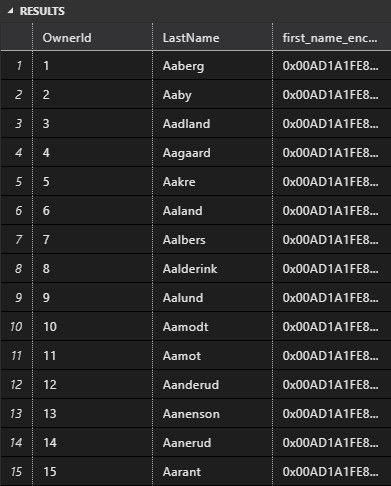
\includegraphics[width=0.8\linewidth]{Prt sc/Figure_1.jpg}  
		\end{minipage}
		\caption{Таблиця відповідності пiдроздiлу та кількості примiщень цього типу.}
	\end{figure}

    Наступна таблиця містить: тип підрозділу, назву цього підрозділу, тип кімнати відповідний
    до цього підрозділу, тип будівлі та дані власника цього будинку. Для отримання потрібних
    даних виконаємо таку команду:
    \begin{lstlisting}[language=SQL]
    SELECT SubdivisionType, SubdivisionName, Rm.TypeOfRoom, Bl.TypeOfBuilding, Ow.FirstName, Ow.LastName
    FROM Subdivision Sub, Room Rm, Building Bl, Ownerss Ow
    WHERE Sub.SubdivisionId = Rm.SubdivisionId AND Rm.BiuldingId=Bl.BiuldingId AND Bl.IdOwner=Ow.OwnerId
    \end{lstlisting}

\newpage
    \begin{figure}[h!]
		\begin{minipage}[h]{1\linewidth}
            \centering
			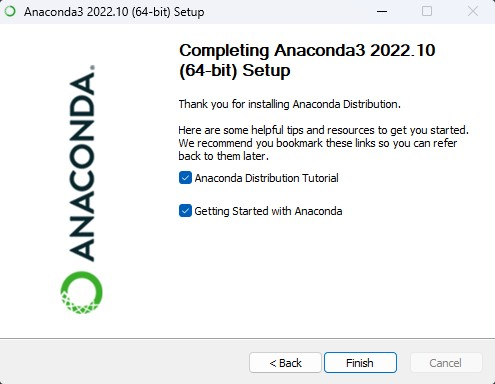
\includegraphics[width=1\linewidth]{Prt sc/Figure_2.jpg}  
		\end{minipage}
		\caption{Результат.}
	\end{figure}

\newpage
    При виникненні питань щодо полів таблиці або реалізації додав код нижче.
    \begin{lstlisting}[language=SQL]
    CREATE DATABASE TestProject
    GO
    USE TestProject
        
    CREATE TABLE Ownerss(
        OwnerId INT IDENTITY(1, 1) PRIMARY KEY,
        FirstName VARCHAR(50) NOT NULL,
        LastName VARCHAR(50) NOT NULL );
        
    CREATE TABLE Building(
        BiuldingId INT IDENTITY(1, 1) PRIMARY KEY CLUSTERED ,
        IdOwner INT NOT NULL,
        TypeOfBuilding VARCHAR(50) NOT NULL,
        AmountOfRooms INT CHECK (AmountOfRooms BETWEEN 1 AND 120),
        AmountOfFloors INT CHECK (AmountOfFloors BETWEEN 1 AND 32),
        CONSTRAINT Error_owner_id FOREIGN KEY (IdOwner) 
        REFERENCES Ownerss (OwnerId) );
        
    CREATE TABLE Subdivision(
        SubdivisionId INT IDENTITY(1, 1) PRIMARY KEY,
        SubdivisionName VARCHAR(50) UNIQUE NOT NULL,
        SubdivisionType VARCHAR(50) NOT NULL );
        
    CREATE TABLE TypeOfSeats(
        SeatsId INT IDENTITY(1, 1) PRIMARY KEY,
        TypeOfSeats VARCHAR(50) UNIQUE NOT NULL ); 
        
    CREATE TABLE Room(
        RoomId INT IDENTITY(1, 1) PRIMARY KEY,
        TypeOfRoom VARCHAR(50) NOT NULL,
        Area INT CHECK (Area BETWEEN 10 AND 70), 
        AmountOfSeats INT CHECK (AmountOfSeats BETWEEN 0 AND 50), 
        RoomNumber INT CHECK (RoomNumber BETWEEN 1 AND 80), 
        SubdivisionId INT,
        BiuldingId INT NOT NULL,
        Storey INT CHECK (Storey BETWEEN 1 AND 32)
        CONSTRAINT Error_subdivision_id FOREIGN KEY (SubdivisionId) 
        REFERENCES Subdivision (SubdivisionId) ON DELETE CASCADE,
        CONSTRAINT Error_biulding_id FOREIGN KEY (BiuldingId) 
        REFERENCES Building (BiuldingId) ON DELETE CASCADE );
        
    CREATE TABLE RoomSeats(
        RoomId INT FOREIGN KEY REFERENCES Room(RoomId),
        SeatsId INT FOREIGN KEY REFERENCES TypeOfSeats(SeatsId),
        PRIMARY KEY(RoomId, SeatsId) );
    \end{lstlisting}

\end{document}